\subsubsection{Testbench và Kết quả mô phỏng Program Counter (PC)}

\textbf{a. Mô tả kịch bản kiểm chứng (Testbench)} \\
Môi trường mô phỏng khối Program Counter được thiết lập nhằm xác minh khả năng quản lý luồng địa chỉ lệnh của CPU. Các kịch bản kiểm thử tập trung vào tính đúng đắn của logic điều khiển và cơ chế ưu tiên tín hiệu:
\begin{itemize}
    \item \textbf{Kiểm tra Reset đồng bộ}: Xác minh \texttt{pc\_out} quay về 0 ngay khi có sườn dương clock tác động trong lúc \texttt{rst} ở mức cao.
    \item \textbf{Kiểm tra tăng địa chỉ (\texttt{inc\_pc})}: Mô phỏng giai đoạn Fetch thông thường, mỗi chu kỳ địa chỉ tăng thêm 1 đơn vị.
    \item \textbf{Kiểm tra nạp địa chỉ (\texttt{ld\_pc})}: Mô phỏng lệnh nhảy (JMP), địa chỉ được nạp trực tiếp từ giá trị toán hạng \texttt{d\_in}.
    \item \textbf{Kiểm tra mức độ ưu tiên}: Kích hoạt đồng thời \texttt{ld\_pc} và \texttt{inc\_pc} để chứng minh hệ thống luôn ưu tiên nạp địa chỉ nhảy trước khi thực hiện tăng tuần tự.
\end{itemize}

\textbf{b. Mã nguồn Testbench (Verilog)}
\begin{lstlisting}[language=Verilog, caption={Ma nguon Testbench kiem tra Program Counter}]
`timescale 1ns / 1ps

module tb_program_counter();

    reg          clk;
    reg          rst;
    reg          ld_pc;
    reg          inc_pc;
    reg  [31:0]  d_in;
    wire [31:0]  pc_out;

    // Khoi tao module PC (Unit Under Test)
    program_counter uut (
        .clk(clk),
        .rst(rst),
        .ld_pc(ld_pc),
        .inc_pc(inc_pc),
        .d_in(d_in),
        .pc_out(pc_out)
    );

    // Tao xung clock chu ky 10ns
    always #5 clk = ~clk;

    initial begin
        // Khoi tao gia tri ban dau
        clk = 0; rst = 0; ld_pc = 0; inc_pc = 0; d_in = 32'b0;

        $display("-------");
        $display("Time|rst|ld_pc|inc_pc|d_in|pc_out");
        $display("-------");
        $monitor("%10t|%b|%b|%b|%h|%h", 
                 $time, rst, ld_pc, inc_pc, d_in, pc_out);

        // 1. Kiem tra Reset
        #12; rst = 1;
        #10; rst = 0;

        // 2. Kiem tra tang dia chi (inc_pc)
        #10; inc_pc = 1; // Tang len 1
        #10; inc_pc = 1; // Tang len 2
        #10; inc_pc = 0; // Dung tang, giu gia tri 2

        // 3. Kiem tra nap dia chi nhay (ld_pc)
        #10; d_in = 32'h0000_0ABC; ld_pc = 1;
        #10; ld_pc = 0; // Giu gia tri 0ABC

        // 4. Tang tu dia chi moi
        #10; inc_pc = 1;
        #10; inc_pc = 0; 

        // 5. Kiem tra uu tien: Vua nap vua tang (ld_pc phai thang)
        #10; d_in = 32'h0000_FFFF; ld_pc = 1; inc_pc = 1;
        #10; ld_pc = 0; inc_pc = 0; 

        #20;
        $display("-------");
        $display("Hoan thanh mo phong Program Counter!");
        $finish;
    end
endmodule
\end{lstlisting}

\textbf{c. Kết quả xuất ra màn hình (Console Output)} \\
Kết quả Console xác nhận PC luôn cập nhật giá trị khớp với các sự kiện điều khiển theo đúng kịch bản mô phỏng.

\begin{figure}[H]
    \centering
    % Thay 'pc_console.png' bang file anh console cua ban
    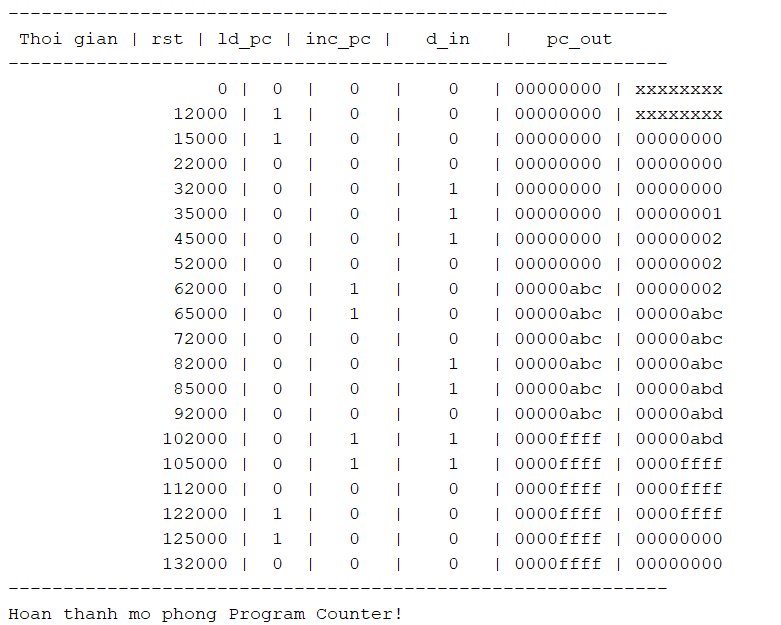
\includegraphics[width=0.8\textwidth]{consolepc.png} 
    \caption{Kết quả chạy Testbench Program Counter trên Console}
    \label{fig:pc_console}
\end{figure}

Dựa trên kết quả \texttt{\$monitor}, tại thời điểm $t=102ns$, khi cả hai tín hiệu \texttt{ld\_pc} và \texttt{inc\_pc} đều ở mức cao, ngõ ra \texttt{pc\_out} đã cập nhật giá trị từ \texttt{d\_in} (0xFFFF). Điều này minh chứng cấu trúc \texttt{if-else} trong module đã thực thi đúng mức ưu tiên thiết kế.

\textbf{d. Giản đồ sóng (Waveform)} \\
Sự thay đổi của bộ đếm PC được thể hiện rõ nét qua giản đồ thời gian, đảm bảo tính đồng bộ hoàn toàn với hệ thống.

\begin{figure}[H]
    \centering
    % Thay 'pc_waveform.png' bang file anh waveform cua ban
    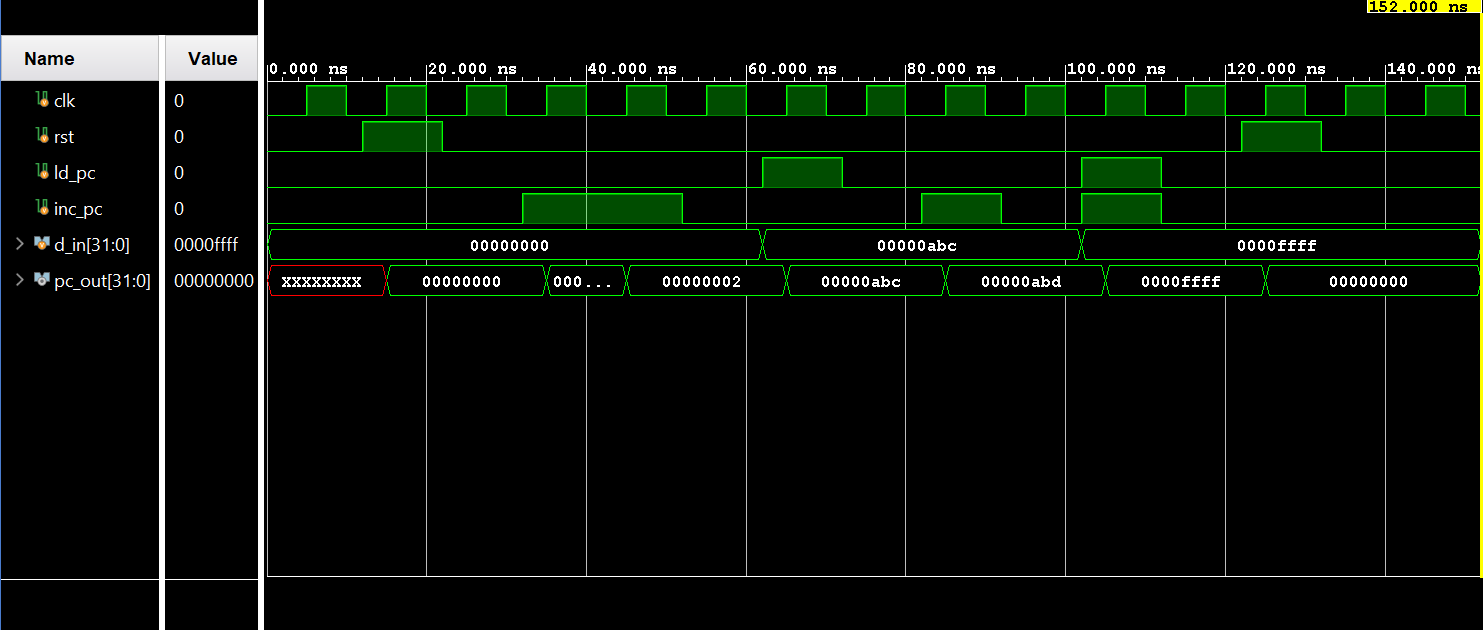
\includegraphics[width=\textwidth]{wavepc.png} 
    \caption{Giản đồ thời gian (Waveform) mô phỏng khối Program Counter}
    \label{fig:pc_waveform}
\end{figure}

Quan sát các sườn dương của xung clock (\texttt{clk}), địa chỉ \texttt{pc\_out} chỉ thay đổi trạng thái khi có sự tác động của \texttt{rst}, \texttt{ld\_pc} hoặc \texttt{inc\_pc}. Các khoảng thời gian còn lại, dữ liệu được duy trì ổn định, giúp việc truy xuất bộ nhớ lệnh không bị sai sót do nhiễu tín hiệu.
\textbf{e. Sơ đồ mạch RTL (RTL Schematic)} \\
Sơ đồ RTL sau khi tổng hợp cho thấy PC được hiện thực bằng các Flip-Flop 32-bit có tích hợp các bộ Mux điều khiển ở ngõ vào để chọn giữa các chế độ: Reset về 0, nạp dữ liệu nhảy hoặc tăng địa chỉ qua bộ cộng (Add Unit).

\begin{figure}[H]
    \centering
    % Nhớ chụp ảnh sơ đồ mạch trong Vivado và đặt tên file là 'pc_rtl.png'
    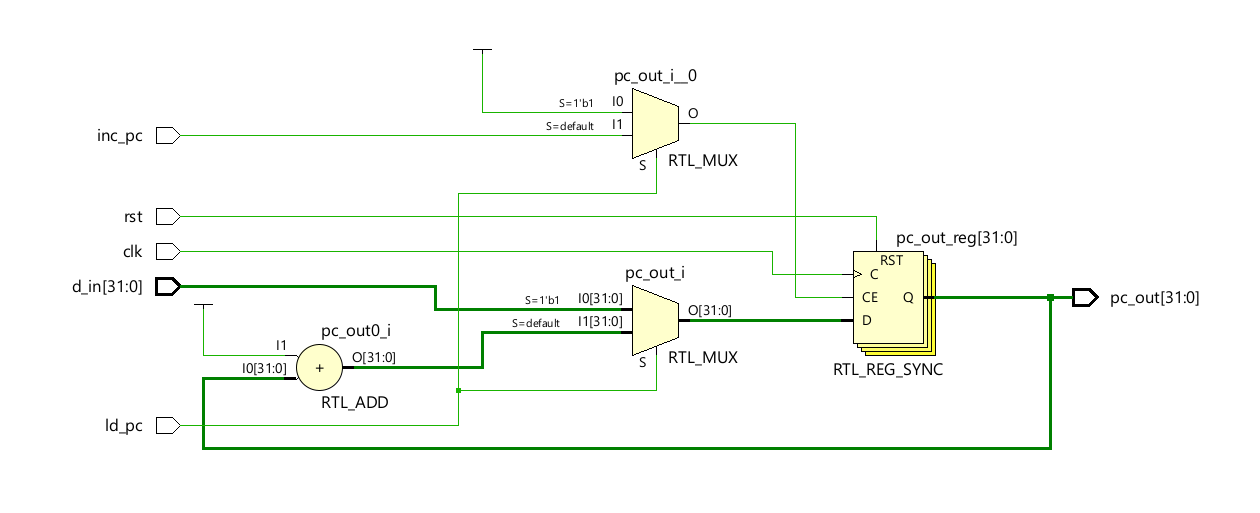
\includegraphics[width=\textwidth]{sodopc.png} 
    \caption{Sơ đồ mạch logic (RTL Schematic) của khối Program Counter}
    \label{fig:pc_rtl}
\end{figure}